\documentclass[12pt]{article}
\usepackage{amsmath}
\usepackage{amsfonts}
\usepackage{graphicx}
\DeclareGraphicsExtensions{.pdf,.png,.jpg}
\usepackage{algpseudocode}

\newtheorem{theorem}{Theorem}[section]
\newtheorem{lemma}[theorem]{Lemma}
\newtheorem{definition}[theorem]{Definition}


\title{Some Questions}
\date{}
\begin{document}
	Say we have a very simple world as shown in Figure \ref{fig:world}. The gray block in the middle is an obstacle. Dotted lines are medial axis. And our algorithm gives some discs. By connecting the centers of these discs, we got a rather sparse road map.\\
	
	If I understand the definition of "retraction" correctly, I simplify the topology of the road map as in Figure \ref{fig:topology}. The second graph in Figure \ref{fig:topology} should be homotopy equivalent to the road map. Suppose we do have an algorithm that is capable of doing the retraction.\\
	
	Now the simplified graph says there are 3 obstacles in the space. It seems this problem cannot be solved, because given 3 circles, you cannot identify if there is any obstacles be tween them. So are 4 and 5 circles. And this is just in a 2D space. It could be worse in 3D or higher dimension.
	
	What can we do with the simplified graph? It seems we can't use it to do motion planning because all points are in one place now. And we cannot use it to say how many obstacles there are, because of the problem above. 
	
	
	
  \begin{figure}[p]
  \centering
  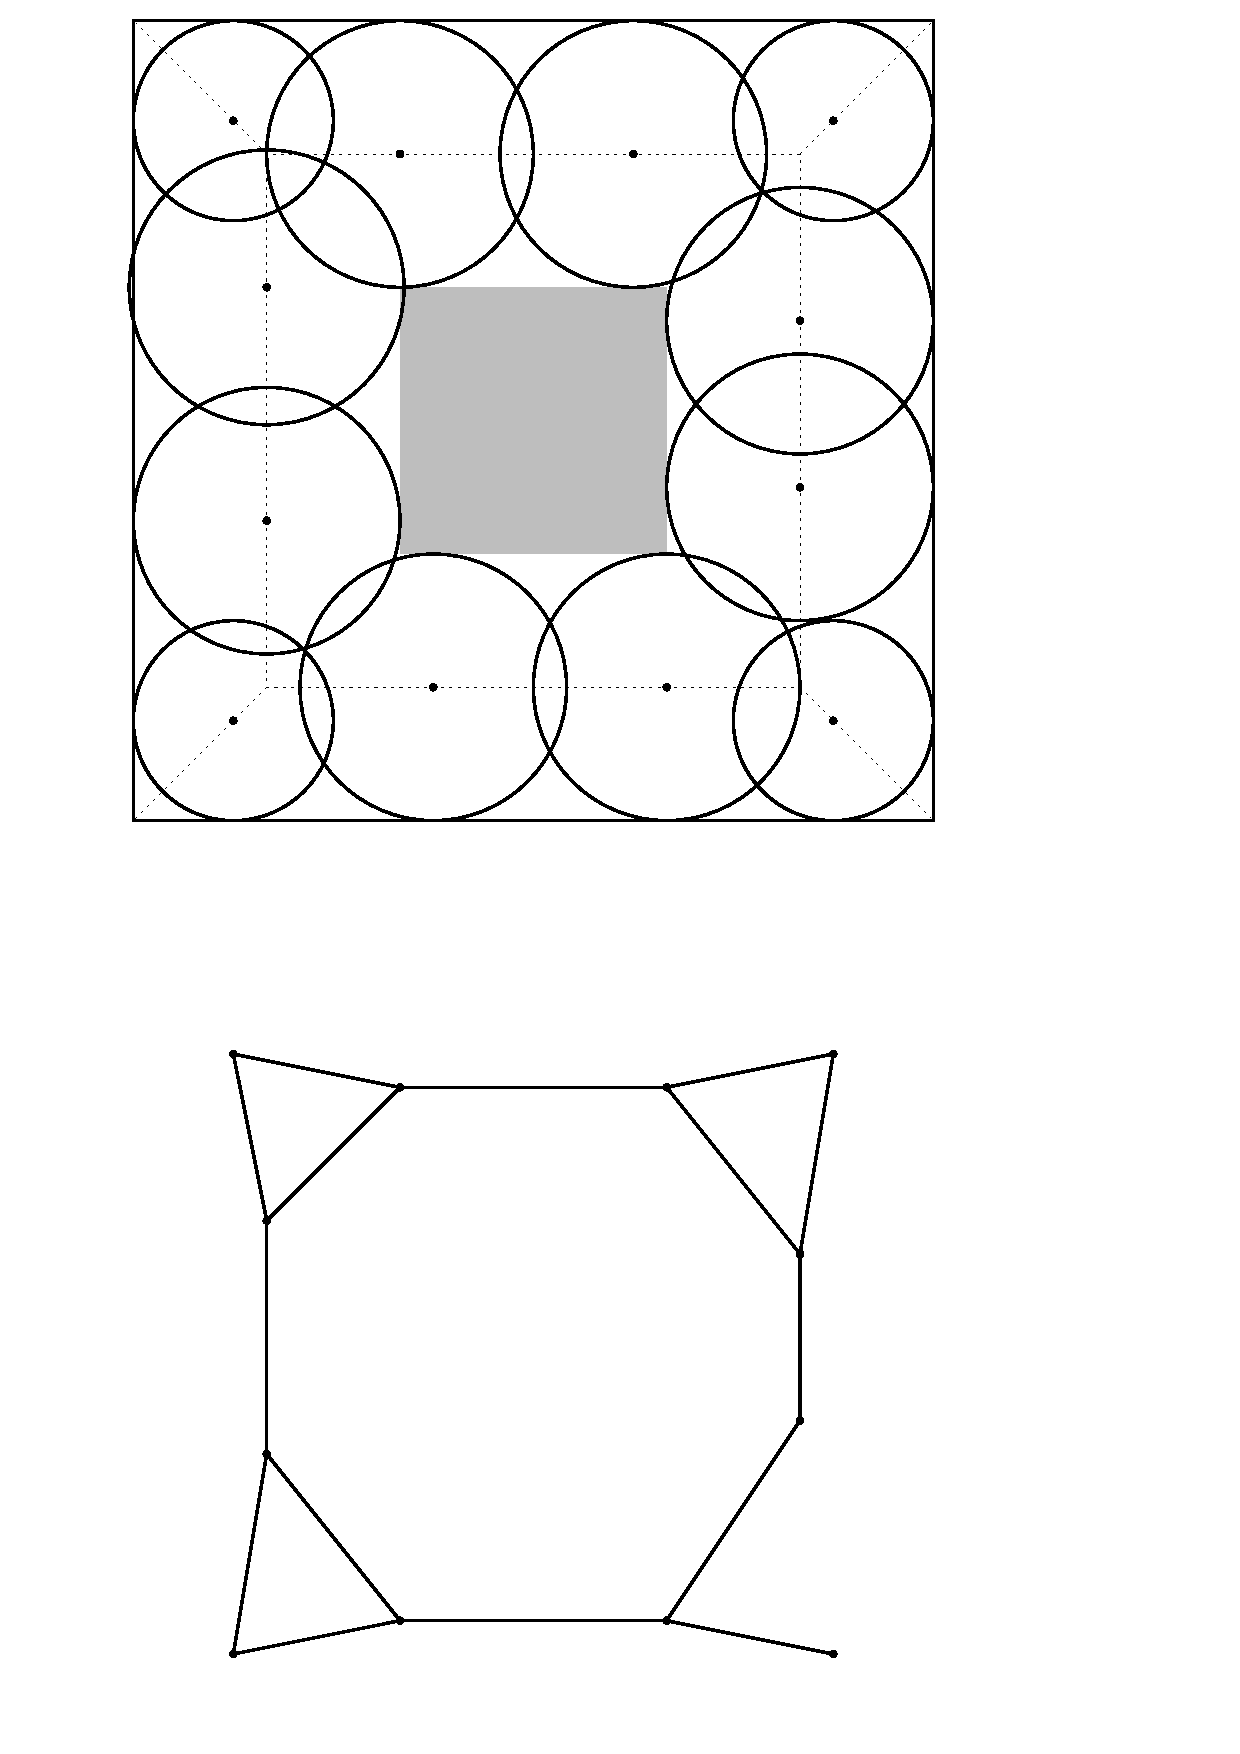
\includegraphics[scale=0.5]{init.pdf}  
  \caption{Simple World and Its road map from MA Sampling }   
  \label{fig:world} 
  \end{figure} 
  
  \begin{figure}[p]
  \centering
  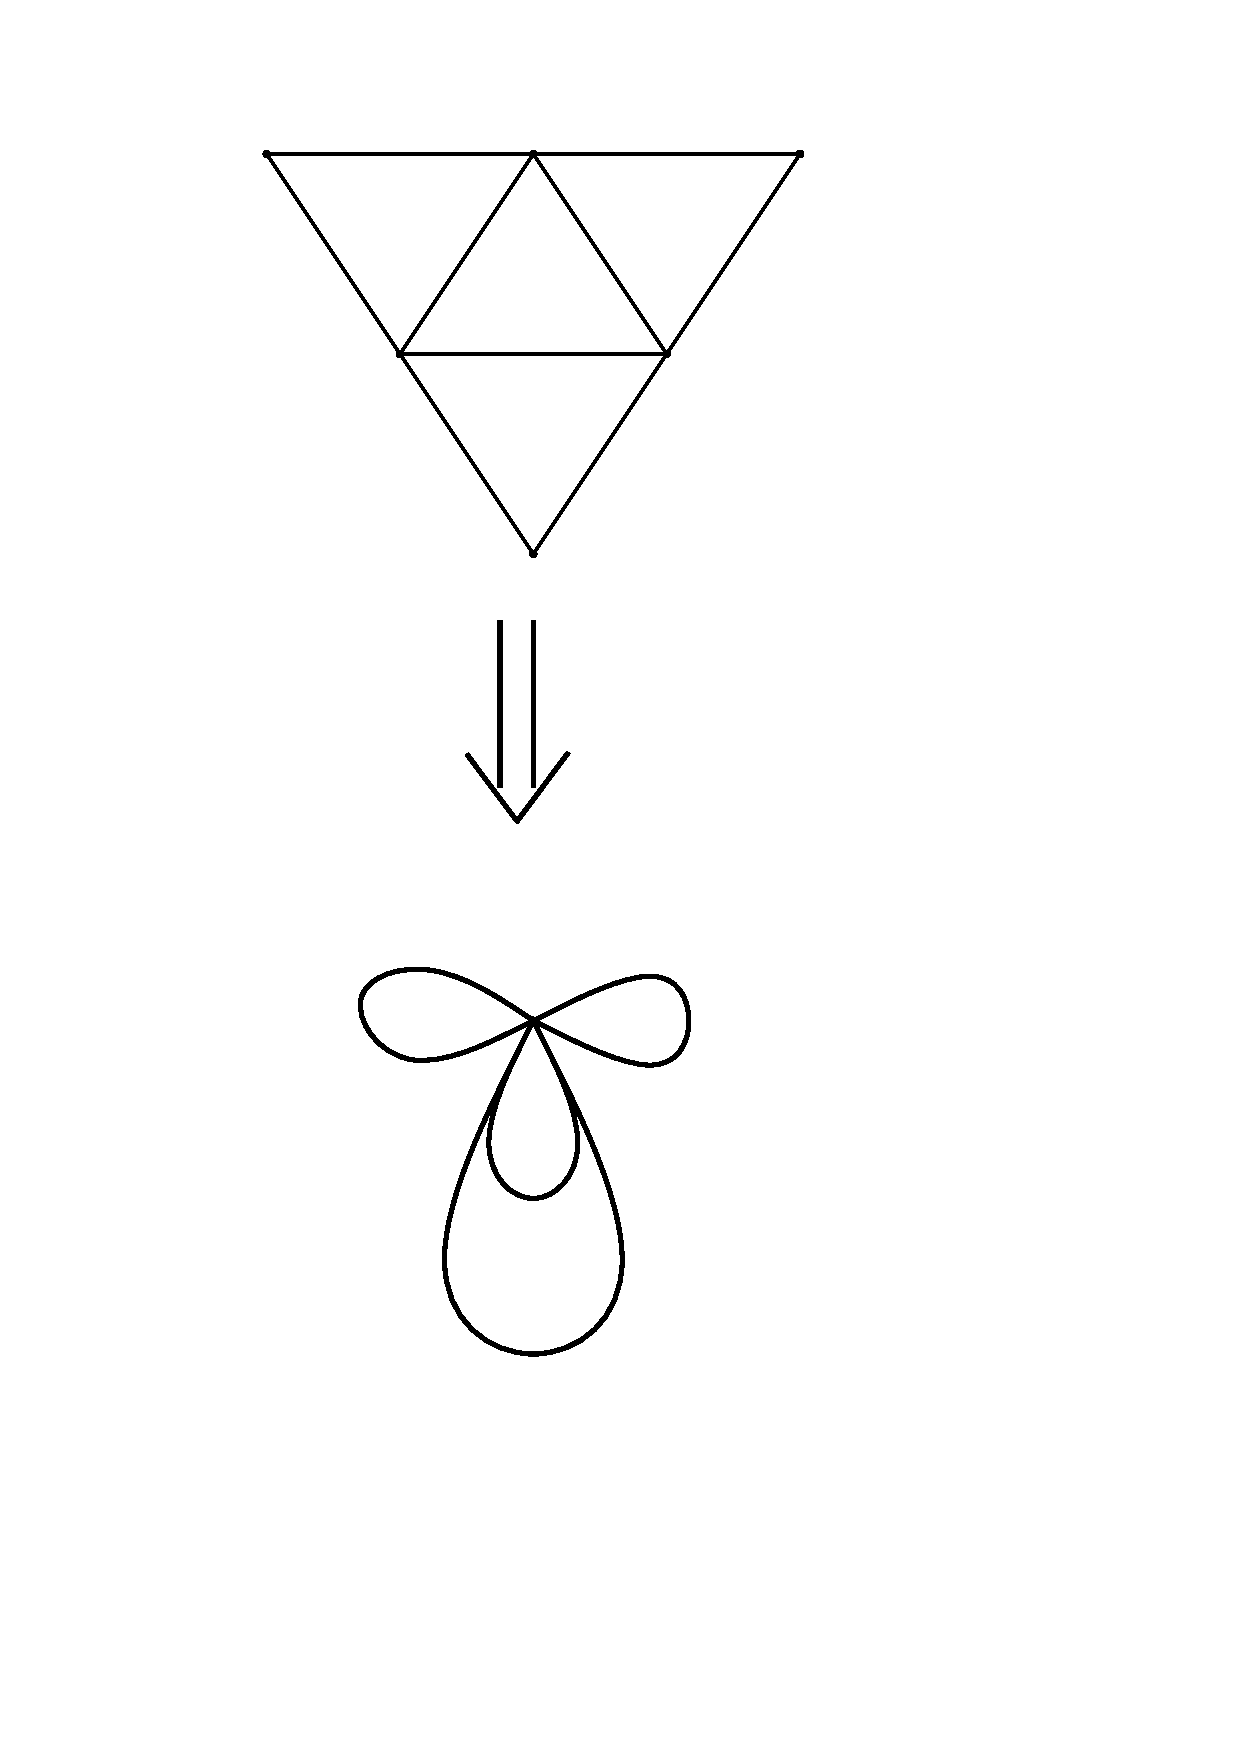
\includegraphics[scale=0.5]{topo.pdf}  
  \caption{Simplified topology}   
  \label{fig:topology} 
  \end{figure} 
\end{document}